\documentclass{article}

\usepackage[utf8]{inputenc}
\usepackage{amsmath}
\usepackage{amssymb}
\usepackage{anysize}
\usepackage{color}
\usepackage{xcolor}
\usepackage{graphicx}
\usepackage{float}

\usepackage{subfigure}

\definecolor{dkgreen}{rgb}{0, 0.6, 0}
\definecolor{gray}{rgb}{0.5, 0.5, 0.5}
\usepackage{listings}
\lstset{
	language=Matlab,                	% choose the language of the code
	keywords={break,case,catch,continue,else,elseif,end,for,function,
      global,if,otherwise,persistent,return,switch,try,while},
      keywordstyle=\color{blue},
      commentstyle=\color{red},
	basicstyle=\footnotesize,       % the size of the fonts that are used for the code
	numbers= left,                 	% where to put the line-numbers
	numberstyle=\footnotesize,      % the size of the fonts that are used for the line-numbers
	stepnumber=1,                   % the step between two line-numbers. If it is 1 each line will be numbered
	numbersep=5pt,                  % how far the line-numbers are from the code
	backgroundcolor=\color{white},  % choose the background color. You must add \usepackage{color}
	showspaces=false,               % show spaces adding particular underscores
	showstringspaces=false,         % underline spaces within strings
	showtabs=false,                 % show tabs within strings adding particular underscores
	frame=single,           		% adds a frame around the code
	tabsize=2,          			% sets default tabsize to 2 spaces
	captionpos=t,          			% sets the caption-position to bottom (t=top, b=bottom)
	breaklines=true,        		% sets automatic line breaking
	breakatwhitespace=false,    	% sets if automatic breaks should only happen at whitespace
	escapeinside={\%*}{*),  % if you want to add a comment within your code
	flexiblecolumns=true}         
}

\usepackage{caption}
\DeclareCaptionFont{white}{\color{white}}
\DeclareCaptionFormat{listing}{\colorbox{gray}{\parbox[c]{\textwidth}{#1#2#3}}}
\captionsetup[lstlisting]{format=listing,labelfont=white,textfont=white}

\setlength\parindent{0pt}
\setlength{\parskip}{10pt}

\marginsize{3cm}{2cm}{2cm}{2cm}

\title{Visual Perception\\
		OpenCV Toolbox\\
		User Manual}
\author{Emre Ozan Alkan\\
		\{emreozanalkan@gmail.com\}\\
		MSCV-5}
\date{\today}

\begin{document}
\maketitle

\section{Introduction}
	Developing Computer Vision applications can be tough. One should consider the capabilities of the framework, on the other hand how this framework will react and perform on given test data. In other case, one may want to see only effect of the consecutive image processing functions on test data. In both and many cases, small toolboxes of the frameworks help people to see results easily, fast and enable them to fast prototyping. Hence this toolbox is created for Computer Vision application developers and enthusiast who want to see image processing functions on their images with very basic knowledge. It's developed with minimal design, which makes it easy to use. However it is also powerful toolbox due to its support of parameters.
	
	
\section{Getting Started}

	\subsection{Basics}
	This application is embedding functions of OpenCV(tested on 2.4.8) for users. This application consist of one main window and sub-windows prompt upon on displaying input and output images by OpenCV. It accepts one image at a time and storing it as original image. Each modification is applied on output image consecutively. There is also history option keep track of change of the output image where you can revert to any old state you want. By default, all operations are disabled until you select an image.
	
	\subsection{User Interface}
	User interface consist of 4 buttons and a tab view which embeds all image processing functions. \par

\begin{figure}[H]
\begin{center}
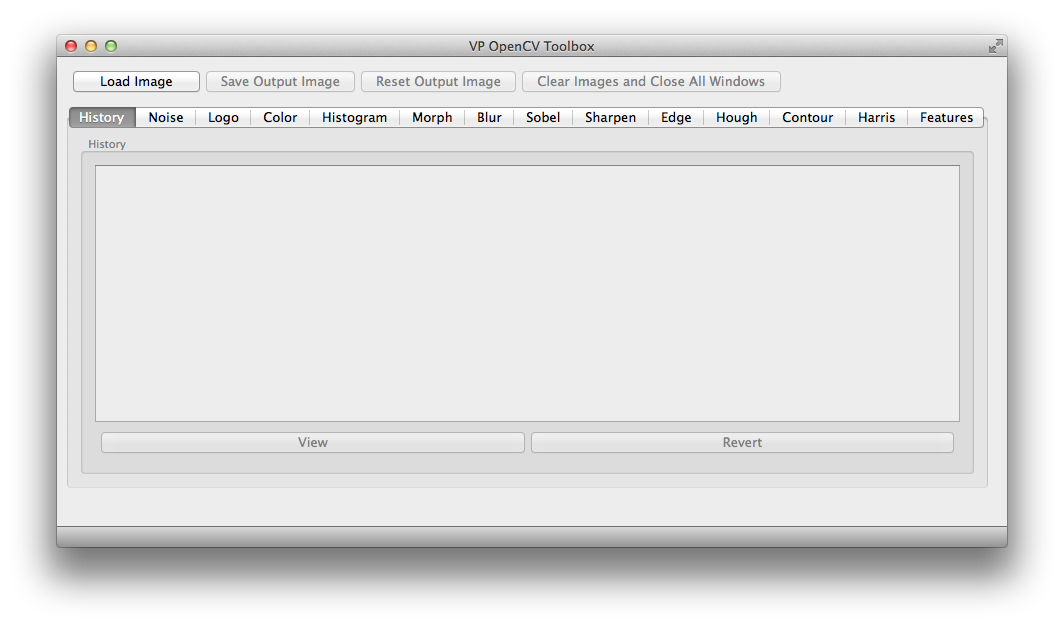
\includegraphics[scale=0.4]{toolbox1.png}
\caption{VP OpenCV Toolbox}
\end{center}
\end{figure}	
	
	Main buttons:
	\begin{itemize}
		\item Load Image: Loads image.
		\item Save Output Image: Saves current output image.
		\item Reset Output Image: Resets output to original loaded image.
		\item Clear Images and Close All WIndows: Clear history stack, output and closes windows.
	\end{itemize}
	
	Tabs:
	\begin{itemize}
		\item History: History of change of output images
		\item Noise: Adding salt and pepper noise
		\item Logo: Adding logo and ROI
		\item Color: Changing color space
		\item Histogram: Calculating and Equalizing Histogram.
		\item Morph: Morphological Operations.
		\item Blur: Blurring operations.
		\item Sobel: Sobel and Laplacian derivative operators.
		\item Sharpen: Sharpening images.
		\item Edge: Canny Edge Detect.
		\item Hough: Hough Transfor finding lines and circles
		\item Contour: Finding countours of connected objects.
		\item Harris: Harris corner extraction.
		\item Features: Extracting FAST, SURF, SIFT key points.
	\end{itemize}

\section{Image Input and Output}

	Image input and output is very easy in this toolbox. "Load Image" button in upper left corner opens file dialog and enable to select any image in your computer. Supported formats are *.png, *.jpg, *.jpeg, amd *.bmp; by default, OpenCV loads images in BGR color space. As soon as you select and load image, image is opened in windows titled "Input", which you can see there is already toolboxes on it which enable you to zoom in/out, showing pixel values and even saving. \par
	Even Qt built OpenCV windows has saving option, there is also saving current image option on left top of application. It opens save dialog and let you save your image any place you want.

\section{Image History}
	Image history is one of the strong functionality of this toolbox. After your each operation, output image is saved and kept for history. \par
	In any moment, you can go history tab and click "Revert" button to go back to that state of the image. Another beautiful feature is  you can see that history items by clicking "View" and they will be pop-up in seperate windows, you can open as much as you want.
	
\begin{figure}[H]
\begin{center}
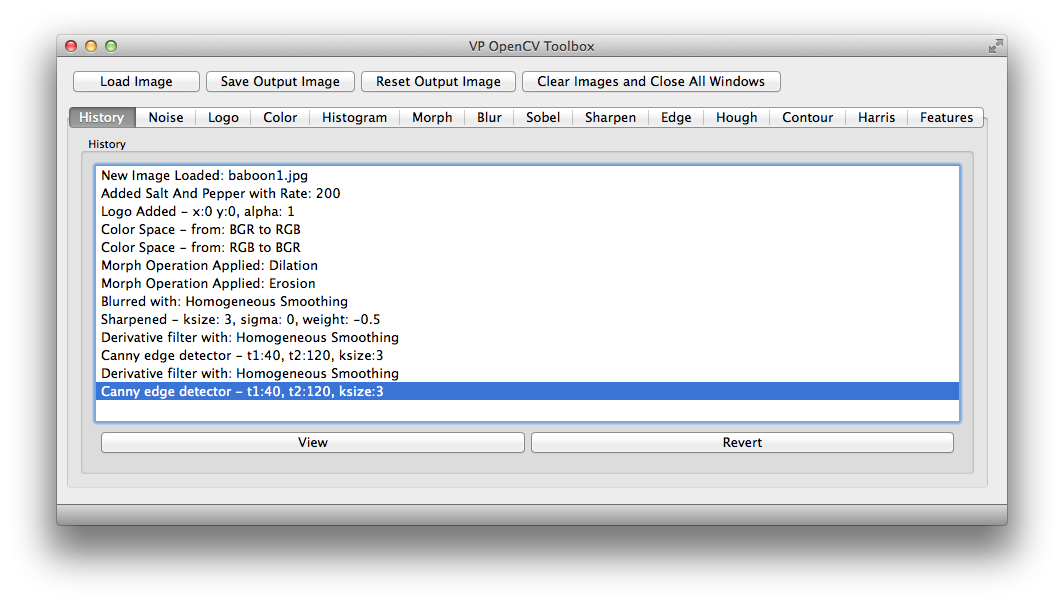
\includegraphics[scale=0.42]{toolboxHistory.png}
\caption{History with Details}
\end{center}
\end{figure}	

\section{Noise}
In "Noise" tab, there is only Salt and Pepper noise option. It's adding white and black pixels to your image with given amount as "Rate" parameter, by default set to 100. Salt and Pepper options are with check-boxes, you have option to add them separately.

\begin{figure}[H]
\begin{center}
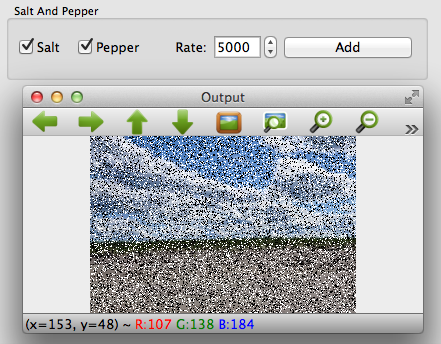
\includegraphics[scale=0.8]{toolboxNoise.png}
\caption{Salt and Pepper Noise}
\end{center}
\end{figure}	

\section{Logo}

In "Logo" tab, first you need to load logo by clicking "Load Logo". You should select logo smaller or equal to output image size, otherwise warning message will appear. Click "Add Logo" to add your logo. There are 5 parameters you can manipulate before adding logo to your image. Here are the parameters:


\begin{table}[H]
\begin{center}
\begin{tabular}{|c|c|l|l|l|}
\hline
\textbf{Parameters} & \multicolumn{4}{|c|}{\textbf{Details}}           \\ \hline
X                  & \multicolumn{4}{|c|}{Logo offset X}              \\ \hline
Y                  & \multicolumn{4}{|c|}{Logo offset Y}              \\ \hline
Alpha              & \multicolumn{4}{|c|}{Weight of the image}        \\ \hline
Beta               & \multicolumn{4}{|c|}{Weight of the logo}         \\ \hline
Gamma              & \multicolumn{4}{|c|}{Scalar added to each pixel} \\ \hline
\end{tabular}
\end{center}
\end{table}

\begin{figure}[H]
\begin{center}
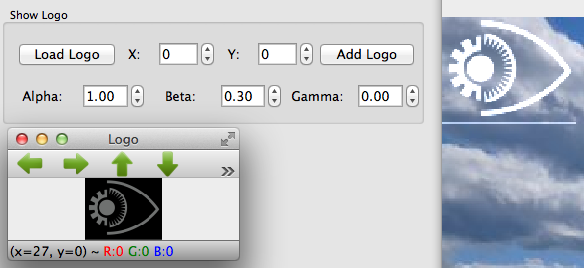
\includegraphics[scale=0.7]{toolboxLogo.png}
\caption{Adding Logo}
\end{center}
\end{figure}	


\section{Color}

In "Color" tab, you can change the color space of the your current image. Supported color spaces are: BGR, RGB, GRAY, HSV, HLS. Current color space combo-box is disabled by default that showing current color space of the image. Each time you change the color space both 'Current Color Space' and 'New Color Space' combo-boxes are updated accordingly.

\begin{figure}[H]
\begin{center}
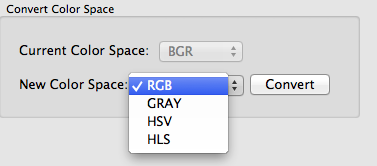
\includegraphics[scale=0.7]{toolboxColorSpace.png}
\caption{Changing Color Space}
\end{center}
\end{figure}	

\section{Histogram}

In "Histogram" tab, you can calculate histogram of the image or equalize histogram of the current image. There is also option to choose channel for viewing histograms for multi channel images. 

\begin{figure}[H]
\begin{center}
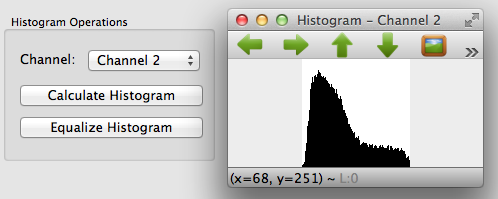
\includegraphics[scale=0.8]{toolboxHistogram.png}
\caption{Histogram Calculation}
\end{center}
\end{figure}	

\section{Morph}

In "Morph" tab, you can perform morphological operations to your current image. Available operations are; Dilation, Erosion, Opening, Closing, Morphological Gradient, Top Hat and Black Hat. Parameters are:

\begin{table}[H]
\begin{center}
\begin{tabular}{|c|c|l|l|l|}
\hline
\textbf{Parameters}  & \multicolumn{4}{|c|}{\textbf{Details}}                                                          \\ \hline
Operation            & \multicolumn{4}{|c|}{Dilation/Erosion/Opening/Closing/Morphological Gradient/Top Hat/Black Hat} \\ \hline
Iteration Count      & \multicolumn{4}{|c|}{Number of times erosion and dilation are applied}                          \\ \hline
Kernel Size          & \multicolumn{4}{|c|}{Size of the structuring element.}                                          \\ \hline
Kernel Type          & \multicolumn{4}{|c|}{Element shape}                                                             \\ \hline
Kernel Anchor X      & \multicolumn{4}{|c|}{x-coordinate of the kernel anchor}                                         \\ \hline
Kernel Anchor Y      & \multicolumn{4}{|c|}{y-coordinate of the kernel anchor}                                         \\ \hline
Image Padding Method & \multicolumn{4}{|c|}{Pixel extrapolation method}                                                \\ \hline
\end{tabular}
\end{center}
\end{table}

\begin{figure}[H]
\begin{center}
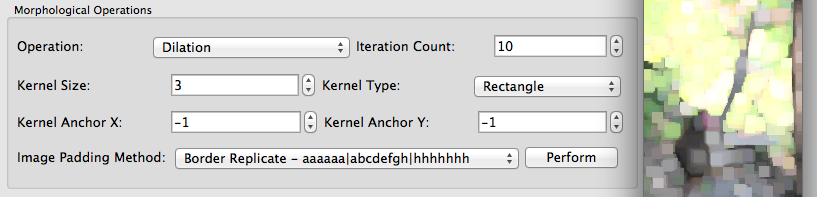
\includegraphics[scale=0.5]{toolboxMorph.png}
\caption{Histogram Calculation}
\end{center}
\end{figure}	

\section{Blur}

In "Blur" tab, you can perform blurring your image with Homogeneous, Gaussian, Median or Bilateral smoothing.You also have options to specify kernel size, its anchor and border replication method. Parameters are:

\begin{table}[H]
\begin{center}
\begin{tabular}{|c|c|l|l|l|}
\hline
\textbf{Parameters}  & \multicolumn{4}{|c|}{\textbf{Details}}                                                          \\ \hline
Bllurring Method            & \multicolumn{4}{|c|}{Homogeneous/Gaussian/Median/Bilateral} \\ \hline
Kernel Size          & \multicolumn{4}{|c|}{Size of the structuring element.}                                          \\ \hline
Kernel Anchor X      & \multicolumn{4}{|c|}{x-coordinate of the kernel anchor}                                         \\ \hline
Kernel Anchor Y      & \multicolumn{4}{|c|}{y-coordinate of the kernel anchor}                                         \\ \hline
Image Padding Method & \multicolumn{4}{|c|}{Pixel extrapolation method}                                                \\ \hline
\end{tabular}
\end{center}
\end{table}

\begin{figure}[H]
\begin{center}
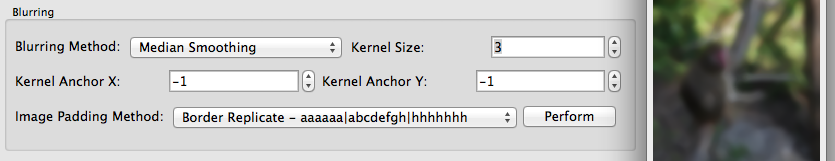
\includegraphics[scale=0.5]{toolboxBlur.png}
\caption{Blurring}
\end{center}
\end{figure}	


\section{Sobel}

In "Sobel" tab, you can use Sobel and Laplacian operators with many parameters.	Parameters are;

\begin{table}[H]
\begin{center}
\begin{tabular}{|c|c|l|l|l|}
\hline
\textbf{}               & \multicolumn{4}{|c|}{\textbf{Details}}                                            \\ \hline
Operation               & \multicolumn{4}{|c|}{Sobel/Laplacian}                                             \\ \hline
Output Depth            & \multicolumn{4}{|c|}{CV\_8U/CV\_16U/CV\_16S/CV\_32F/CV\_64F}                      \\ \hline
Image Padding Method    & \multicolumn{4}{|c|}{Pixel extrapolation method.}                            \\ \hline
Sobel Kernel Size       & \multicolumn{4}{|c|}{size of the extended Sobel kernel; it must be 1, 3, 5, or 7} \\ \hline
Sobel X Order           & \multicolumn{4}{|c|}{Order of the derivative x}                                   \\ \hline
Sobel Y Order           & \multicolumn{4}{|c|}{Order of the derivative y}                                   \\ \hline
Scale Factor            & \multicolumn{4}{|c|}{Optional scale factor for the computed derivative values;}   \\ \hline
Delta Offset            & \multicolumn{4}{|c|}{Optional delta value that is added to the results}           \\ \hline
Laplacian Aperture Size & \multicolumn{4}{|c|}{Aperture size used to compute the second-derivative filters} \\ \hline
\end{tabular}
\end{center}
\end{table}


\begin{figure}[H]
\begin{center}
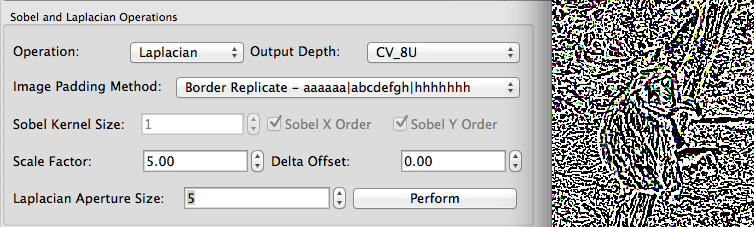
\includegraphics[scale=0.5]{toolboxSobel.png}
\caption{Laplacian Operator}
\end{center}
\end{figure}	


\section{Sharpen}
In "Sharpen" tab, you can perform sharpening on images. Behind the code, gaussian blurred image is weighted with the current image. Parameters are:

\begin{table}[H]
\begin{center}
\begin{tabular}{|c|c|l|l|l|}
\hline
\textbf{Parameters}  & \multicolumn{4}{|c|}{\textbf{Details}}                   \\ \hline
Kernel Size          & \multicolumn{4}{|c|}{Gaussian kernel size}               \\ \hline
Gaussian Sigma       & \multicolumn{4}{|c|}{Gaussian kernel standard deviation} \\ \hline
Image Padding Method & \multicolumn{4}{|c|}{Pixel extrapolation method} \\ \hline
Filter Weight        & \multicolumn{4}{|c|}{Weight of the first array elements} \\ \hline
\end{tabular}
\end{center}
\end{table}


\begin{figure}[H]
\begin{center}
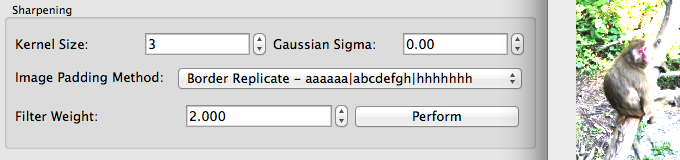
\includegraphics[scale=0.5]{toolboxSharpen.png}
\caption{Sharpening}
\end{center}
\end{figure}	

\section{Edge}
In "Edge" tab, you can use Canny Edge detector algorithm to find edges in your image. There are 4 parameters for Canny. Parameters are:

\begin{table}[H]
\begin{center}
\begin{tabular}{|c|c|l|l|l|}
\hline
\textbf{Parameters} & \multicolumn{4}{|c|}{\textbf{Details}}                                                              \\ \hline
Threshold1          & \multicolumn{4}{|c|}{First threshold for the hysteresis procedure}                                  \\ \hline
Threshold1          & \multicolumn{4}{|c|}{Second threshold for the hysteresis procedure}                                 \\ \hline
Aperture Size       & \multicolumn{4}{|c|}{Aperture size for the Sobel() operator}                                        \\ \hline
L2gradient          & \multicolumn{4}{|c|}{Use l2 normalization should be used to calculate the image gradient magnitude} \\ \hline
\end{tabular}
\end{center}
\end{table}



\begin{figure}[H]
\begin{center}
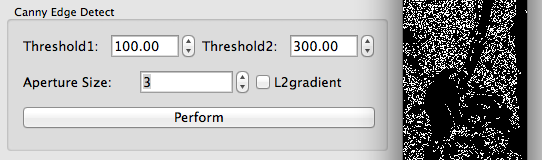
\includegraphics[scale=0.5]{toolboxEdge.png}
\caption{Canny Edge Detector}
\end{center}
\end{figure}	

\section{Hough}
In "Hough" tab, you can find lines and circles with Hough Transform method. By choosing find method Lines or Circles, related parameters are enabled or disabled. Parameters are:

\begin{table}[H]
\begin{center}
\begin{tabular}{|c|c|l|l|l|}
\hline
\multicolumn{5}{|c|}{\textbf{Find Circle}}                                                                                                                                                      \\ \hline
\textbf{Parameters}    & \multicolumn{4}{|c|}{\textbf{Details}}                                                                                                                                 \\ \hline
Threshold              & \multicolumn{4}{|c|}{Accumulator threshold parameter}                                                                                                                  \\ \hline
Theta                  & \multicolumn{4}{|c|}{Angle resolution of the accumulator in radians}                                                                                                   \\ \hline
Rho                    & \multicolumn{4}{|c|}{Distance resolution of the accumulator in pixels}                                                                                                 \\ \hline
SRN                    & \multicolumn{4}{|c|}{For the multi-scale Hough transform, it is a divisor for the distance resolution rho}                                                             \\ \hline
STN                    & \multicolumn{4}{|c|}{For the multi-scale Hough transform, it is a divisor for the distance resolution theta}                                                           \\ \hline
\multicolumn{5}{|c|}{\textbf{Find Circle}}                                                                                                                                                      \\ \hline
\textbf{Parameters}    & \multicolumn{4}{|c|}{\textbf{Details}}                                                                                                                                 \\ \hline
DP                     & \multicolumn{4}{|c|}{Inverse ratio of the accumulator resolution to the image resolution}                                                                              \\ \hline
Min Dist               & \multicolumn{4}{|c|}{Minimum distance between the centers of the detected circles}                                                                                     \\ \hline
Param1                 & \multicolumn{4}{|c|}{First method-specific parameter.}      \\ \hline
Param2                 & \multicolumn{4}{|c|}{Second method-specific parameter} \\ \hline
Min Radius             & \multicolumn{4}{|c|}{Minimum circle radius}                                                                                                                            \\ \hline
Max Radius             & \multicolumn{4}{|c|}{Maximum circle radius}                                                                                                                            \\ \hline
\end{tabular}
\end{center}
\end{table}

\begin{figure}[H]
\begin{center}
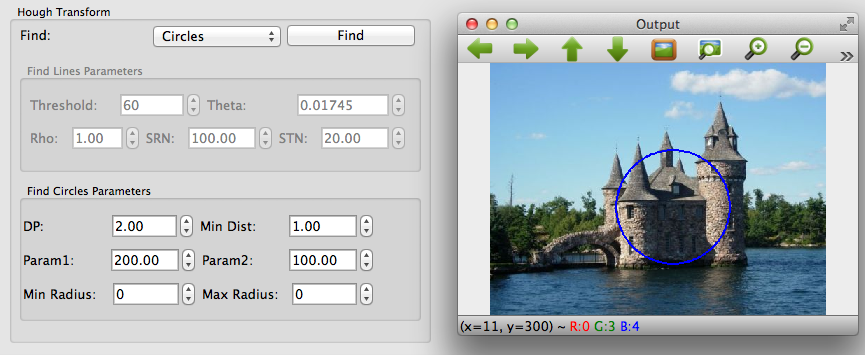
\includegraphics[scale=0.5]{toolboxHough.png}
\caption{Hough Transform}
\end{center}
\end{figure}	

\section{Contour}
In "Contour" tab, you can find contours of connected object and draw them onto image. There are many parameters available. Parameters are:

\begin{table}[H]
\begin{center}
\begin{tabular}{|c|c|l|l|l|}
\hline
\textbf{Parameters} & \multicolumn{4}{|c|}{\textbf{Details}}                                        \\ \hline
Mode                & \multicolumn{4}{|c|}{Contour retrieval mode}                                  \\ \hline
Method              & \multicolumn{4}{|c|}{Contour approximation method}                            \\ \hline
Offset X            & \multicolumn{4}{|c|}{Optional offset by which every contour point is shifted} \\ \hline
Offset Y            & \multicolumn{4}{|c|}{Optional offset by which every contour point is shifted} \\ \hline
Binary Threshold    & \multicolumn{4}{|c|}{Binary threshold value before finding contour}           \\ \hline
Min Contour Size    & \multicolumn{4}{|c|}{Eliminate too short or too long contours}                \\ \hline
Max Contour Size    & \multicolumn{4}{|c|}{Eliminate too short or too long contours}                \\ \hline
Bounding Box        & \multicolumn{4}{|c|}{Drawing bounding box}                                    \\ \hline
Bounding Min Cirle  & \multicolumn{4}{|c|}{Drawing bounding circle}                                 \\ \hline
\end{tabular}
\end{center}
\end{table}


\begin{figure}[H]
\begin{center}
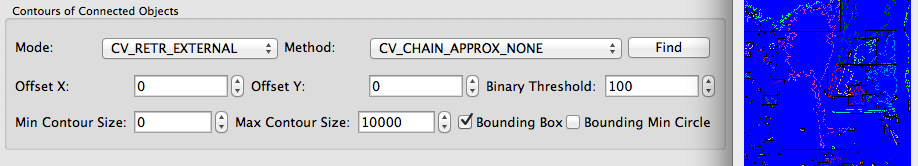
\includegraphics[scale=0.5]{toolboxContours.png}
\caption{Contours}
\end{center}
\end{figure}	

\section{Harris}
Tn "Harris" tab, you can extract corners with Harris Corner Extraction. Parameters are:

\begin{table}[H]
\begin{center}
\begin{tabular}{|c|c|l|l|l|}
\hline
\textbf{Parameters}             & \multicolumn{4}{|c|}{\textbf{Details}}                              \\ \hline
Derivative Size of Neighborhood & \multicolumn{4}{|c|}{Neighborhood size}                             \\ \hline
Harris Parameter                & \multicolumn{4}{|c|}{Harris detector free parameter}                \\ \hline
Non-max Size of Neighborhood    & \multicolumn{4}{|c|}{Aperture parameter for the Sobel() operator}   \\ \hline
Image Padding Method            & \multicolumn{4}{|c|}{Pixel extrapolation method}                    \\ \hline
Threshold Max Strength          & \multicolumn{4}{|c|}{Binary threshold value before finding contour} \\ \hline
\end{tabular}
\end{center}
\end{table}

\begin{figure}[H]
\begin{center}
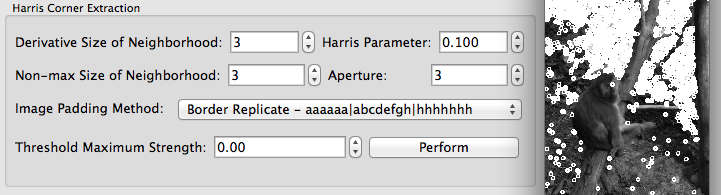
\includegraphics[scale=0.5]{toolboxHarris.png}
\caption{Contours}
\end{center}
\end{figure}	           

\section{Features}
In "Features" tab you can find 3 method implemented for keypoint extraction from current image.

\begin{figure}[H]
\begin{center}
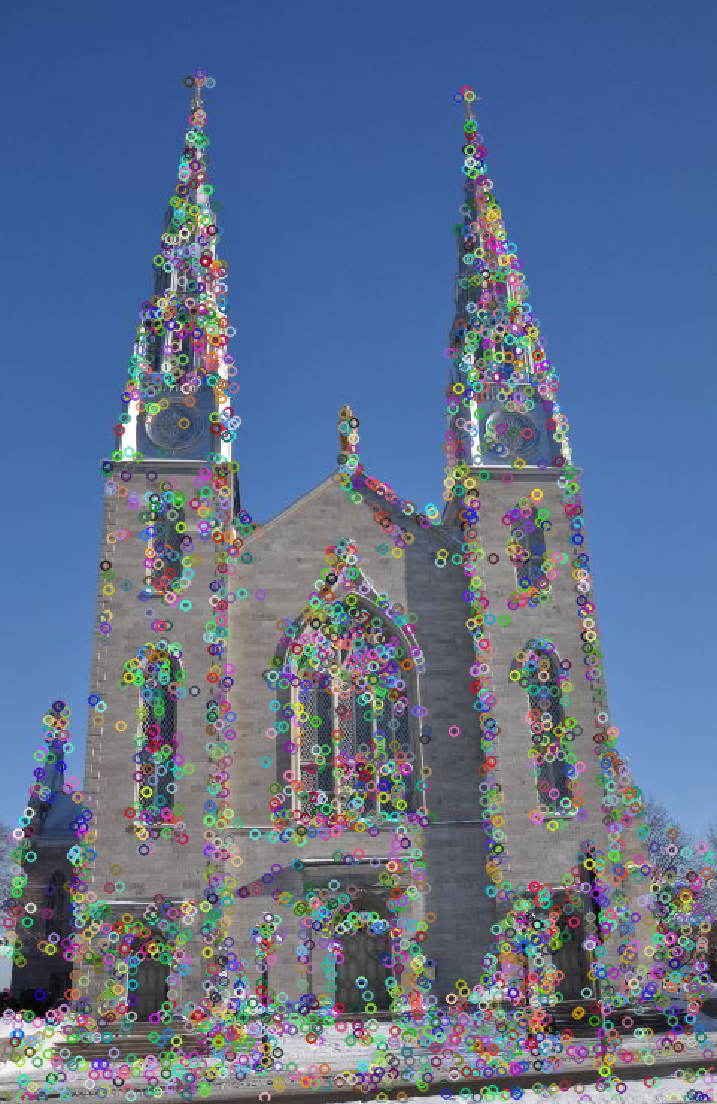
\includegraphics[scale=0.3]{toolboxFeature.png}
\caption{SIFT Keypoint Extraction}
\end{center}
\end{figure}	   

	\subsection{FAST}
	Using "FastFeatureDetector" and given parameters, it finds key points. Parameters are:

\begin{table}[H]
\begin{center}
\begin{tabular}{|c|c|l|l|l|}
\hline
\textbf{Parameters}   & \multicolumn{4}{|c|}{\textbf{Details}}                                                                                        \\ \hline
Threshold             & \multicolumn{4}{|c|}{Threshold on diff between intensity of the central pixel} \\ \hline
Non-max Supression    & \multicolumn{4}{|c|}{If true, non-maximum suppression is applied to detected corners (keypoints)}                             \\ \hline
Keypoint Drawing Flag & \multicolumn{4}{|c|}{Flags setting drawing features}                                                                          \\ \hline
Keypoint Colors       & \multicolumn{4}{|c|}{Draws keypoints with different colors}                                                                   \\ \hline
\end{tabular}
\end{center}
\end{table}
	
	\subsection{SURF}
	Using "SurfFeatureDetector" and given parameters, it finds key points. Parameters are:
	
\begin{table}[H]
\begin{center}
\begin{tabular}{|c|c|l|l|l|}
\hline
\textbf{Parameters}   & \multicolumn{4}{|c|}{\textbf{Details}}                                                                                        \\ \hline
Min Hessian           & \multicolumn{4}{|c|}{Threshold on diff between intensity of central px and px of a circle around this px} \\ \hline
Keypoint Drawing Flag & \multicolumn{4}{|c|}{Flags setting drawing features}                                                                          \\ \hline
Keypoint Colors       & \multicolumn{4}{|c|}{Draws keypoints with different colors}                                                                   \\ \hline
\end{tabular}
\end{center}
\end{table}
	
	
	\subsection{SIFT}
	Using "SiftFeatureDetector" and given parameters, it finds key points. Parameters are:
	
\begin{table}[H]
\begin{center}
\begin{tabular}{|c|c|l|l|l|}
\hline
\textbf{Parameters}   & \multicolumn{4}{|c|}{\textbf{Details}}                                                                \\ \hline
Feature Threshold     & \multicolumn{4}{|c|}{The contrast threshold used to filter out weak features in semi-uniform regions} \\ \hline
Edge Threshold        & \multicolumn{4}{|c|}{The threshold used to filter out edge-like features.}                            \\ \hline
Keypoint Drawing Flag & \multicolumn{4}{|c|}{Flags setting drawing features}                                                  \\ \hline
Keypoint Colors       & \multicolumn{4}{|c|}{Draws keypoints with different colors}                                           \\ \hline
\end{tabular}
\end{center}
\end{table}

\section{Estimation}
In "Estimation" tab, you can find many functions, including camera calibration with chessboard patter, finding matches between images. drawing epipolar lines, connecting two images with tomography and more.

\subsection{Camera Calibration}
Camera calibration is calculating the distortion for your camera and, find undistortion for better image acquire. Parameters are:

\begin{table}[H]
\begin{center}
\begin{tabular}{|c|c|l|l|l|}
\hline
\textbf{Parameters} & \multicolumn{4}{|c|}{\textbf{Details}}                                            \\ \hline
\# Corners X        & \multicolumn{4}{|c|}{Number of corners in horizontal your chessboard pattern has} \\ \hline
\# Corners Y        & \multicolumn{4}{|c|}{Number of corners in vertical your chessboard pattern has}   \\ \hline
\end{tabular}
\end{center}
\end{table}


\begin{figure}[H]
\begin{center}
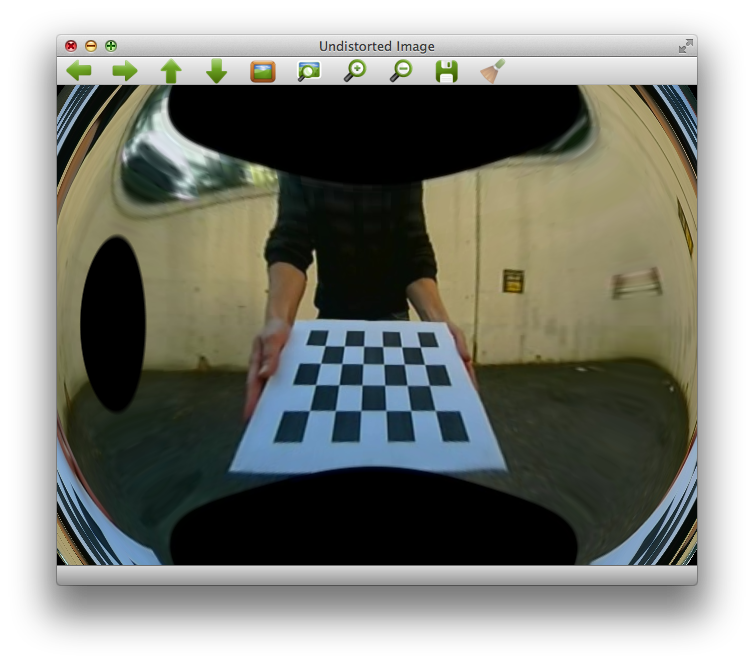
\includegraphics[scale=0.3]{toolboxCameraCalibration.png}
\caption{Undistorted Image After Calibration}
\end{center}
\end{figure}	   

\subsection{Find Matches}
Find matches between two images; current output image and matching image you will provide with "Load Matching Image". Parameters are:

\begin{table}[H]
\begin{center}
\begin{tabular}{|c|c|l|l|l|}
\hline
\textbf{Parameters}          & \multicolumn{4}{|c|}{\textbf{Details}}                                             \\ \hline
SURF Min Hessian             & \multicolumn{4}{|c|}{Threshold on diff between intensity of the central pixel}  \\ \hline
Calculate Fundemental Matrix & \multicolumn{4}{|c|}{Calculates F matrix with given method}    \\ \hline
Keypoint Drawing Flag        & \multicolumn{4}{|c|}{Flags setting drawing features}                               \\ \hline
Matching Image               & \multicolumn{4}{|c|}{Maching image your provide with "Load Matching Image" button} \\ \hline
\end{tabular}
\end{center}
\end{table}

\begin{figure}[H]
\begin{center}
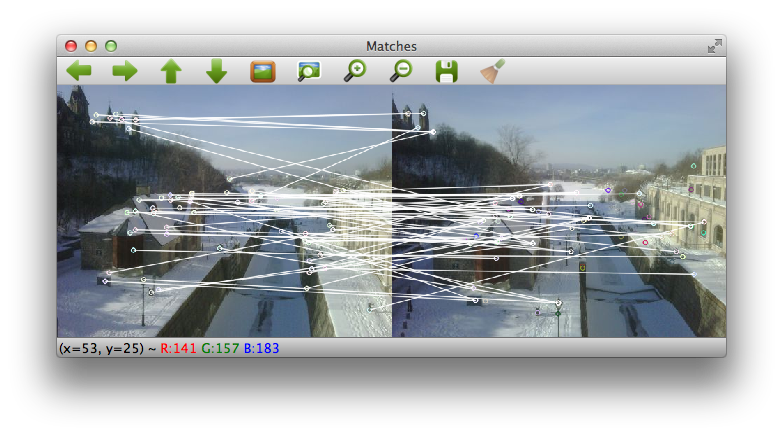
\includegraphics[scale=0.5]{toolboxFindMatches.png}
\caption{Find Matches}
\end{center}
\end{figure}	   

\subsection{Epipolar}
Finds and draws epipolar lines between two images; current output image and matching image you will provide with "Load Matching Image". Parameters are:

\begin{table}[H]
\begin{center}
\begin{tabular}{|c|c|l|l|l|}
\hline
\textbf{Parameters}      & \multicolumn{4}{|c|}{\textbf{Details}}                                                                    \\ \hline
Ratio                    & \multicolumn{4}{|c|}{Max ratio between 1st and 2nd Nearest Neighbor}                                      \\ \hline
SURF Min Hessian         & \multicolumn{4}{|c|}{Threshold on diff between intensity of central px and px of a circle around this px} \\ \hline
Confidence Level         & \multicolumn{4}{|c|}{Confidence level (probability)}                                                      \\ \hline
Min Distance to Epioplar & \multicolumn{4}{|c|}{Min distance to epipolar}                                                            \\ \hline
Matching Image           & \multicolumn{4}{|c|}{Maching image your provide with "Load Matching Image" button}                        \\ \hline
\end{tabular}
\end{center}
\end{table}

\begin{figure}[H]
\begin{center}
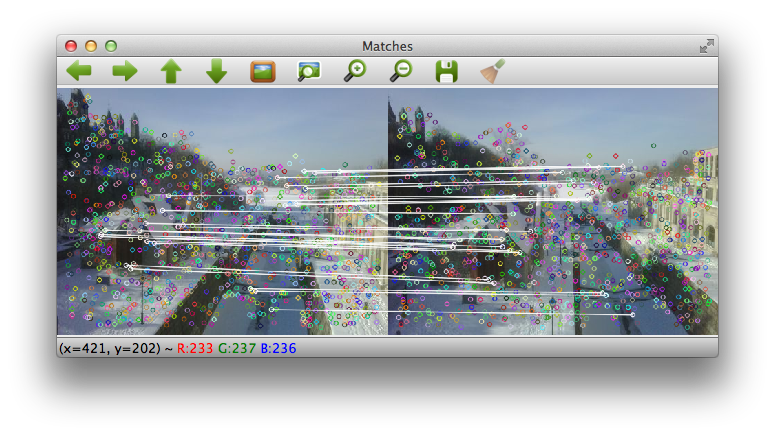
\includegraphics[scale=0.5]{toolboxEpipolarLines.png}
\caption{Epipolar Lines}
\end{center}
\end{figure}	   


\subsection{Homography}
Computes the homography between two images and connect them by the found homography. Parameters are:

	\begin{table}[H]
\begin{center}
\begin{tabular}{|c|c|l|l|l|}
\hline
\textbf{Parameters}      & \multicolumn{4}{|c|}{\textbf{Details}}                                                                    \\ \hline
Ratio                    & \multicolumn{4}{|c|}{Max ratio between 1st and 2nd Nearest Neighbor}                                      \\ \hline
SURF Min Hessian         & \multicolumn{4}{|c|}{Threshold on diff between intensity of central px and px of a circle around this px} \\ \hline
Confidence Level         & \multicolumn{4}{|c|}{Confidence level (probability)}                                                      \\ \hline
Min Distance to Epioplar & \multicolumn{4}{|c|}{Min distance to epipolar}                                                            \\ \hline
Matching Image           & \multicolumn{4}{|c|}{Maching image your provide with "Load Matching Image" button}                        \\ \hline
\end{tabular}
\end{center}
\end{table}

\begin{figure}[H]
\begin{center}
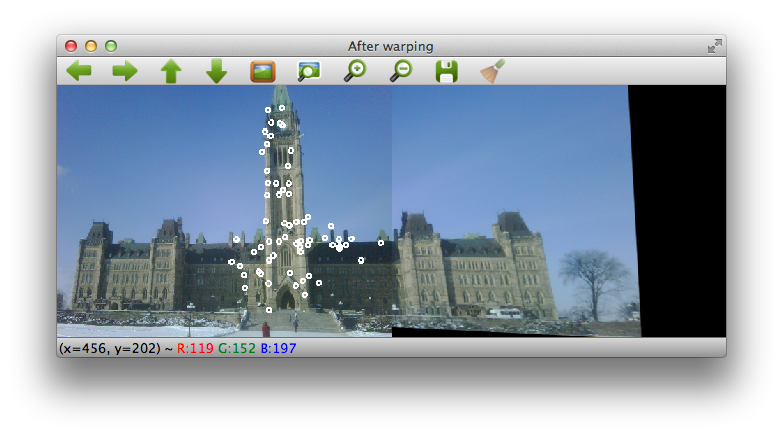
\includegraphics[scale=0.5]{toolboxHomography.png}
\caption{Homography Applied Image}
\end{center}
\end{figure}	   

\end{document}
